\documentclass{article}

% if you need to pass options to natbib, use, e.g.:
% \PassOptionsToPackage{numbers, compress}{natbib}
% before loading nips_2016
%
% to avoid loading the natbib package, add option nonatbib:
%\usepackage[nonatbib]{nips_2016}

\usepackage[final]{nips_2016}

% to compile a camera-ready version, add the [final] option, e.g.:
% \usepackage[final]{nips_2016}

\usepackage[utf8]{inputenc} % allow utf-8 input
\usepackage[T1]{fontenc}    % use 8-bit T1 fonts
\usepackage{hyperref}       % hyperlinks
\usepackage{url}            % simple URL typesetting
\usepackage{booktabs}       % professional-quality tables
\usepackage{amsfonts}       % blackboard math symbols
\usepackage{nicefrac}       % compact symbols for 1/2, etc.
\usepackage{microtype}      % microtypography
\usepackage{multirow}
\usepackage{graphicx}
\usepackage{siunitx}
\usepackage{placeins}

\bibliographystyle{plainnat}
\setcitestyle{numbers,square}

\graphicspath{ {./figures} }

\title{Comparing Convolutional Neural Networks and Vision Transformers for Image Classification}

\author{
  Krist\'of K\'assa \\  
  Budapest University \\
  of Technology and Economics\\
  \texttt{kassak@edu.bme.hu}
  \And
  Lilla Barancsuk \\
  Budapest University \\ 
  of Technology and Economics\\
  \texttt{barancsuk.lilla@vik.bme.hu} \\
}


\begin{document}

\maketitle

\begin{abstract}
Convolution Neural Network (CNN) algorithms have been prominent models for image classification, but in recent years Transformer based methods have also started to gain popularity. In an attempt to get a clear view and understanding of the two architectures for image classification tasks on a cloud dataset of approximately 2000 data points, a framework was designed to compare the characteristics of CNN and Vision Transformer (ViT) for image classification. For each model we provide a comprehensive review of architectural and functional differences. Then we compare their computing capacity requirements, validation accuracy and training time on an online image dataset with our own implementation of input pipeline from scratch.
\end{abstract}

\section{Introduction}
The Convolutional Neural Network (CNN) is a sub-type of Neural Networks. CNN \cite{Krizhevsky2012,LeCun1989} models are exceedingly well suited for image recognition and classification applications due to their built-in convolutional layer(s) aiming to reduce the high dimensionality of images without any information loss. The architecture is based upon the idea that one pixel of the given picture is dependent on its nearby pixels (brightness, color or contrast). Therefore, a CNN based algorithm can extract important low/mid/high level features \cite{Zeiler2014} and edges by applying filters on specific subsets of the given image in a convolutional manner. 

The Vision Transformer (ViT) architecture however, adopts the mechanism of self-attention, differentially weighting the significance of each part of the input data and used primarily in the field of natural language processing (NLP) \cite{Vaswani2017}. The use of transformers in computer vision is still limited, although recent studies showed that transformers can be successfully applied for various image processing tasks. 

The goal of this group work is to gain thorough understanding of each architecture to learn about their strengths and limitations.

\section{Related work}
Transformers were proposed by Dosovitskiy et al. in \cite{Dosovitskiy2021} for image classification with supervised machine learning. Comparison of results of ViT against CNN architectures on various datasets shows that despite of the fact that ViT requires considerably more computational resources, it can provide better performance for some datasets upon certain training conditions than CNN models. In fact, they showed that the chances of the model performing better are higher if filtering is not applied for extraction but the entire image is processed by the model (as in ViT). As a result, numerous studies were formed to replace CNN with ViT in real-world applications \cite{Bazi2021,Karimi2021}.

\section{Methodology\label{sec:meth}}
\subsection{Dataset}
For our study, we used the Swimcat-extend dataset \cite{Swimcat2020} for cloud image classification. The dataset contains 2100 images of 6 different types of sky conditions, considering cloudiness: Clear Sky, Patterned Clouds, Thin White Clouds, Thick White Clouds, Thick Dark Clouds, Veil Clouds. Before streaming them into our models --- 5 different configurations for both CNN and transformer architectures --- all images are normalized and reshaped to a size of 224x224. Given the small size and class similarity of our cloud dataset we apply K-fold Cross Validation for each CNN and transformer model training to comprehensively evaluate their performance.

\subsection{Data augmentation}
To prevent overfitting, diversify the training set and artificially increase the amount of training data, we apply data augmentation. We define 3 distinct levels (none, low, high) of data augmentation to analyze the effect of augmentation on our model accuracy. While low augmentation layer performs random rotation, high augmentation layer performs rotation, flip, and zoom, as detailed below. For those models where we apply high data augmentation during the learning process, we expect greater robustness and generally improved accuracy and performance. 

\subsection{Neural network architectures}
To compare the two network architectures, four pretrained CNN and ViT models were selected for our test framework. To analyze the effects of parameter count we have chosen 2--2 different models in complexity --- number of parameters  \num{5d6} and \num{d7} --- for the CNN and transformer models both.

\subsubsection{CNN models}
The first selected clonvolutional network model is \textit{EfficientNetB1} which uses a technique called 'Compound Scaling' during its learning process, i.e.,~uniformly scales all dimensions of depth, width and resolution using a compound coefficient, unlike conventional practice that arbitrary scales these factors \cite{Tan2019}. The parameter count of EfficientNet is approximately \num{d7}.

The second model is \textit{ResNet18D}. This model utilizes an average pooling tweak for down sampling. Instead of hoping each few stacked layers directly fit a desired underlying mapping, residual nets let these layers fit a residual mapping. They stack residual blocks on top of each other to form the network \cite{He2016}. The parameter count of this model is about \num{5d6}.

\subsubsection{Transformer models}
Similarly to CNNs, two vision transformer architectures were selected. They are both a variation of the original Vision Transformer model proposed by Dosovitskiy et al.~in \cite{Dosovitskiy2021}. Both models are trained on ImageNet-21k, at a resolution of 224x224 pixels. Model details are seen in Table \ref{tab:vit_models}.

\begin{table}
\centering
\caption{The analyzed Vision Transformer models.\label{tab:vit_models}}
\begin{tabular}{|l|c|c|}
\hline
Model name & Approximate parameter count & Patch size \\ \hline
\textit{vit\_tiny\_patch16\_224} & \num{5d6} & 16 \\ \hline
\textit{vit\_tiny\_r\_s16\_p8\_224\_in21k} &  \num{d7} & 88 \\ \hline
\end{tabular}
\end{table}

\subsubsection{Frozen vs.~trainable weights in the pretrained models}
To kick-start the training, we employed transfer learning \citep{Vilalta2011}. In our study, using transfer learning is necessary, since we do not have a large enough dataset for achieving a good performance on a model trained from scratch.
Prior to utilizing them in our study, both CNN and ViT architectures were pretrained on the ImageNet-21k dataset \citep{Deng2009} for image classification. To analyze the effects of trainable parameter count, for some of our experiments, the pretrained base layer weights were frozen, while for other experiments, the base layers were were left trainable (Table \ref{tab:exp}.).

\subsection{Model structure}
The resulting models consist of the following layers:

\begin{itemize}\setlength{\itemsep}{0.2ex}
\item    Input layer
\item    Optional augmentation layer
\item    Pretrained model (CNN or ViT, trainable or frozen)
\item    Dropout layer for increasing robustness
\item    Dense output layer
\end{itemize}

To increase robustness, an additional dropout layer is added, and for extracting features for the classification, a trainable dense layer was placed on top of the pretrained models in each case.
    
\subsection{5-fold cross-validation}
K-fold cross-validation is a technique used for evaluating machine learning models. The method splits the input dataset into distinct $K$ sample sets, and trains the network separately for each set. This technique can increase the reliability of the performance evaluation and can predict the outcome of unseen data, thus offers a less biased evaluation. For our analysis, 5-fold cross-validation is used.


\section{Experiments}
Using the model, size and augmentation variations described in section \ref{sec:meth}., we compiled 10 experiments with distinct hyper-parameter configurations as seen in Table \ref{tab:exp}.
We trained each model defined in Table \ref{tab:exp}., 5-fold on the entire cloud dataset, and saved categorical accuracy and loss scores throughout the training process.

\begin{table}[]
\caption{Parameter configurations for the experiments performed. \label{tab:exp}}
\begin{tabular}{|l|l|c|c|c|c|}
\hline
 & \textbf{Parameter count} & \multicolumn{1}{l|}{\textbf{Trainability}} & \multicolumn{1}{l|}{\textbf{Augmentation}} & \textbf{CNN model name}         & \textbf{ViT model name}         \\ \hline \hline
                   1  &  \multirow{2}{*}{\textbf{\num{5d6}}}  & \multirow{2}{*}{frozen} & none                                  & cnn\_5m\_f\_na  & vit\_5m\_f\_na   \\\cline{4-6}
2 &  &   & low                                   & cnn\_5m\_f\_la  & vit\_5m\_f\_la  \\\cline{4-6}
               2 &     &  & high                                  & cnn\_5m\_f\_ha  & vit\_5m\_f\_ha  \\\hline
4 & \num{5d6}          & trainable                                    & high                         & cnn\_5m\_t\_ha  & vit\_5m\_t\_ha  \\ \hline
5 & \num{d7}          & trainable                                   & high                         & cnn\_10m\_t\_ha & vit\_10m\_t\_ha \\ \hline
\end{tabular}
\end{table}

\section{Results}
\subsection{Loss and accuracy curve analysis}
Figures \ref{fig:curves_acc},\ref{fig:curves_loss} shows the validation accuracy and loss respectively of the ViT and CNN networks for the five configurations. Curves show an average and deviation across the 5 training runs. Solid lines shows the mean, and the shaded region is related to the empirical standard deviation.
Trainable networks show a more rapid learning compared to frozen models. The main difference between the ViT and CNN result, is that the latter converges faster. On the other hand, CNNs show a higher level of uncertainty in terms of accuracy.
Interestingly, models with low level of augmentation seem to perform better on the validation set. This is due to a strong similarity in the images of the validation set. To mitigate this problem, the models were evaluated using an unseen test dataset, as presented in section \ref{sec:test}.

\begin{figure}[h]
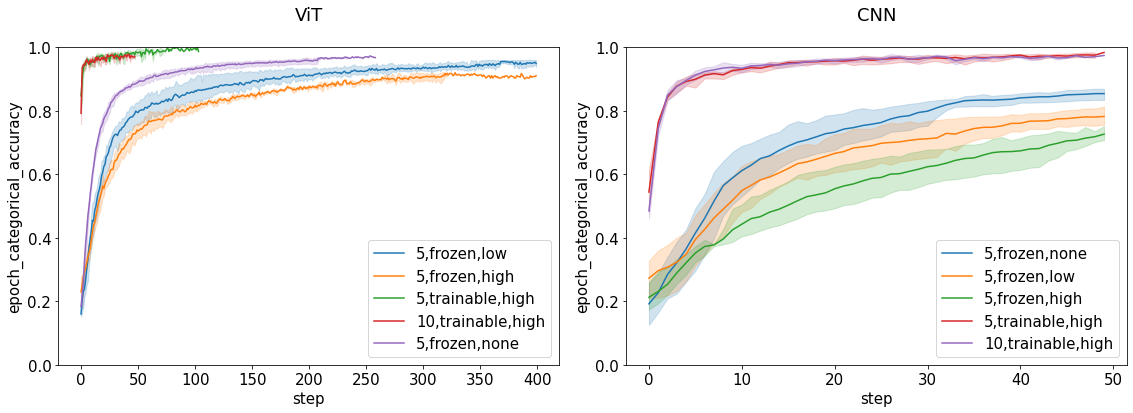
\includegraphics[width=0.9\textwidth]{accuracy_validation.png}
\caption{Categorical accuracy of the validation set during training.\label{fig:curves_acc}}
\end{figure}

\begin{figure}[h]
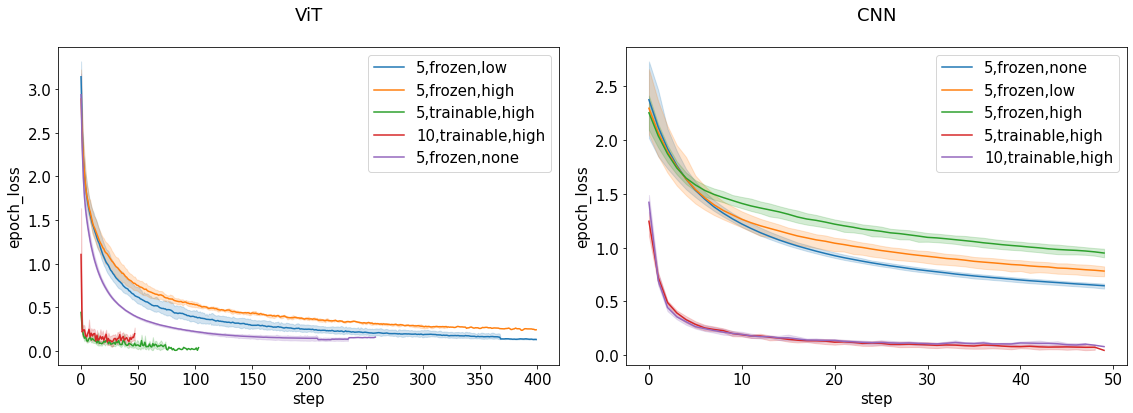
\includegraphics[width=0.9\textwidth]{loss_validation.png}
\caption{Categorical crossentropy of the validation set during training.\label{fig:curves_loss}}
\end{figure}

\subsection{Comparing model performances}
Figures \ref{fig:comp_acc}.,\ref{fig:comp_loss}~ compares the validation accuracy and loss respectively of the models on the training dataset. For this analysis the minimum loss and maximum accuracy were selected from each training run. Trainable models significantly outperform the frozen models. CNN models show a higher loss and lower accuracy compared to ViT, but the difference is less significant for the trainable models. There is no significant difference in terms of model size. The results show, that the most relevant parameter with respect to performance is trainability.

\begin{figure}[h]
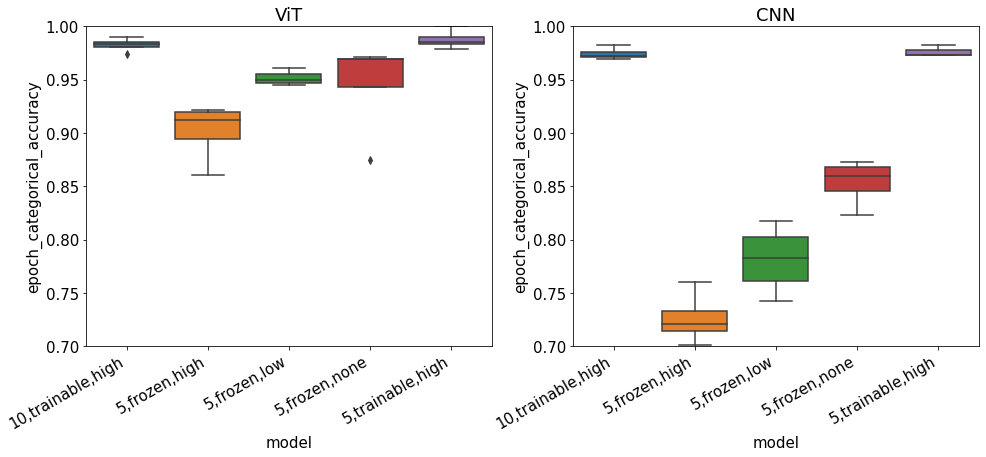
\includegraphics[width=0.9\textwidth]{accuracy_comp_validation.png}
\caption{Maximum categorical accuracy of the validation set during training\label{fig:comp_acc}}
\end{figure}

\begin{figure}[h]
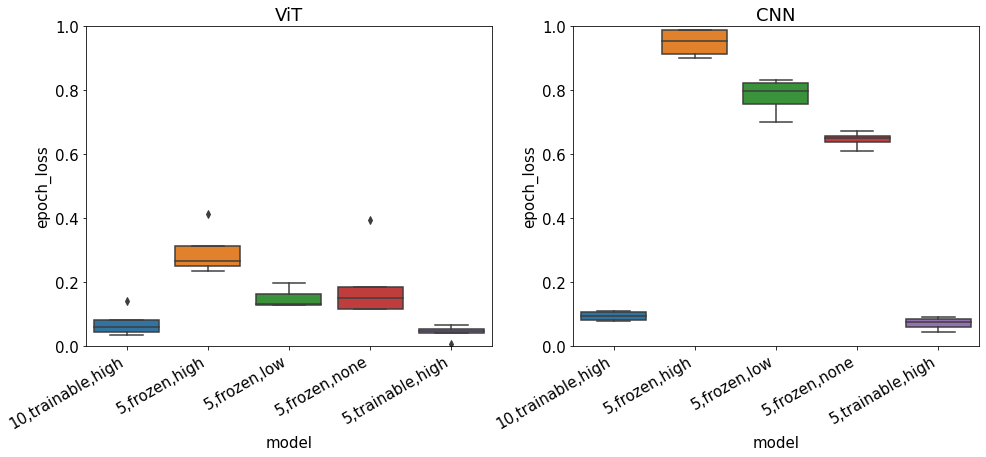
\includegraphics[width=0.9\textwidth]{loss_comp_validation.png}
\caption{Minimum categorical crossentropy of the validation set during training\label{fig:comp_loss}}
\end{figure}

\subsection{Classification accuracy using an independent test set}\label{sec:test}
To test the accuracy of the models on an unseen set of images, independent from the training data, a collection of cloud images was compiled using online sources and our own photos. The test set contains 163 images manually sorted into the 6 classes. For each model, the iteration of the 5-fold cross validation with the best performance (minimum loss) was selected and evaluated. The resulting loss and accuracy scores are shown in Table \ref{tab:test_comp}.

The best ViT model (\SI{77.3}{\%}) outperforms the best CNN model (\SI{74.2}{\%}) in terms of test accuracy. According to our results considering categorical accuracy, loss and computational performance during training and validation, the best architecture for our purpose is $vit\_tiny\_r\_s16\_p8\_224\_in21$ with high level of augmentation.

On the test set, high augmentation models strongly outperform low augmentation ones, showing the importance of training data variability.

\begin{table}[]
\centering
\caption{Comparing the performance of the models using an independent test set.\label{tab:test_comp}}
\begin{tabular}{|l|c|c|}
\hline
\textbf{model} & \textbf{accuracy [\%]} & \textbf{loss} \\ \hline \hline
\textbf{vit\_10m\_ha\_t} & \num{77}                              & \num{1.52}                          \\
\textbf{cnn\_5m\_ha\_t}  & \num{74}                              & \num{1.12}                          \\
\textbf{vit\_5m\_ha\_t}  & \num{72}                              & \num{1.67}                          \\
\textbf{cnn\_10m\_ha\_t} & \num{63}                              & \num{1.20}     \\
\textbf{vit\_5m\_ha\_f}  & \num{56}                              & \num{1.60} \\
\textbf{vit\_5m\_la\_f}  & \num{50}                             & \num{2.56} \\
\textbf{vit\_5m\_na\_f}  & \num{43}                              & \num{3.42} \\
\textbf{cnn\_5m\_na\_f}  & \num{42}                              & \num{1.60} \\
\textbf{cnn\_5m\_ha\_f}  & \num{39}                              & \num{1.60} \\
\textbf{cnn\_5m\_la\_f}  & \num{37}                              & \num{1.61}
 \\ \hline
\end{tabular}
\end{table}

\section{Conclusion and discussion}
This group work proved the applicability and effectiveness of Transformer for image classification tasks. We compared CNN and ViT models with our cloud image dataset. Meanwhile, we have applied different levels of data augmentation to improve model accuracy and used K-fold cross validation to compensate the size of our dataset and to compare the performance of models at scale. 

However, this study still has some limitations. As indicated, the training time for the ViT model is extremely long compared to the CNN models. Therefore, to implement in real-life applications its efficiency must be improved, which needs to be investigated. This work also only studies one type of dataset with limited number of CNN and Transformer models. Other CNN models such as VGGs and Inception-ResNets could be further studied to compare the performance between CNN and ViT models. 

\FloatBarrier

\bibliography{bibliography}
	

\end{document}
